\chapter{THEORETICAL FRAMEWORK}
\normalsize{In this chapter, the basics of fusion such as nuclear physics and magnetic confinement are explained. In addition to that, the construction and the different systems of the W7-X are also explained to give an overview on the device and its auxiliary components. Heat transfer theory as well as solid mechanics including plasticity and fatigue constitute the basis of the work and the complex equations of these theories solved using Finite Element Analysis. These theories are necessary for the completion of this work and are therefore reminded in this chapter.}
\section{GENERAL THEORY OF FUSION REACTORS}
\normalsize{The principle of a nuclear fusion power plant is to make the energy released by the fusion of light atomic nuclei usable. Nuclear fusion which represent the fusing of atomic nuclei together is only achievable if they come close enough to surpass the electrostatic repulsion forces and have the strong nuclear force fuse the nucleons together. Due to electrostatic repulsion forces also called Coulomb barrier, the nuclei repulse each other thus preventing the reaching of the necessary distance (because the strong nuclear force has a very limited range, ~$10^{-15}$m) \cite{diekmann_energie:_2014}\cite{Freidberg_2007} for fusion. Furthermore, the repulsion forces increase with the number of protons in the nucleus or its size. The energy required to fuse two nuclei become subsequently greater.}
\\
\begin{figure}[h!]
    \label{fig_2_1} 
    \centering
    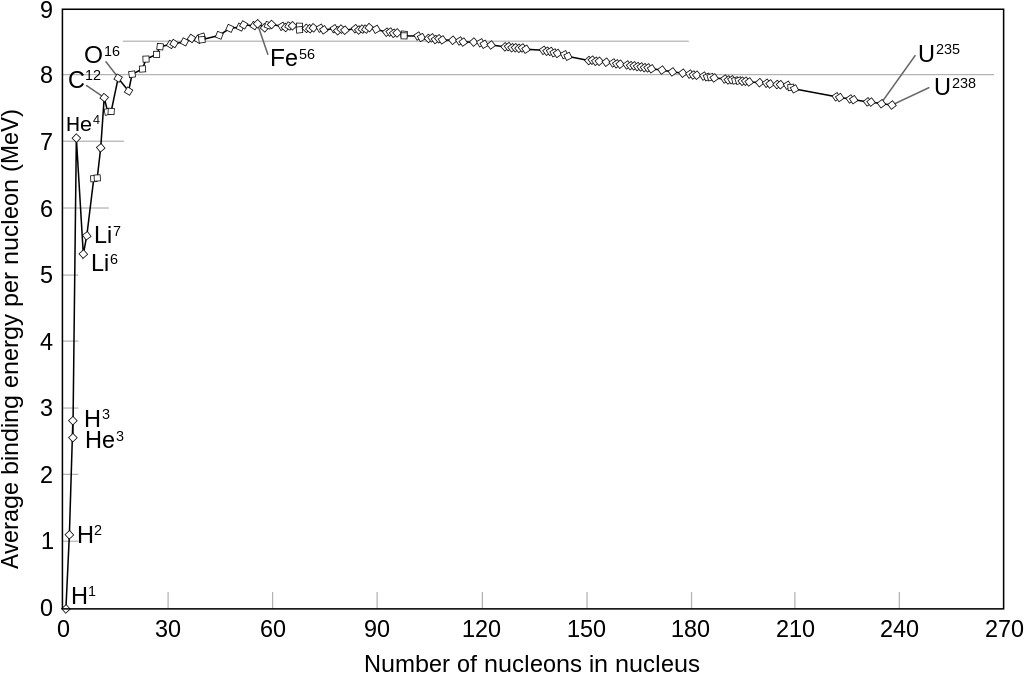
\includegraphics[width=.9\textwidth]{figures/fig_1.png}
    \caption{\it Nuclear binding energy vs. mass number.}
\end{figure}
\\
\normalsize{\indent The different nuclear reactions for transforming hydrogen into helium are \cite{diekmann_energie:_2014}:}
\begin{equation}
    \ce{^1_1H + ^1_0n -> ^2_1H + 2.22 MeV}
\end{equation}
\begin{equation}
    \ce{^2_1H + ^1_1p -> ^3_2He + 5.49 MeV}
\end{equation}
\normalsize{\indent or}
\begin{equation}
    \ce{^2_1H + ^2_1H -> ^3_2He + ^1_0n + 3.27 MeV}
\end{equation}
\begin{equation}
    \ce{^2_1H + ^2_1H -> ^3_1He + ^1_1p + 4.03 MeV}
\end{equation}
\begin{equation}
    \ce{^2_1H + ^3_1H -> ^4_2He + ^1_0n + 17.58 MeV}
\end{equation}
\\
\normalsize{\indent On Figure \ref{fig:fig_2_2}, the cross section for various reactions are graphed in function of the ion temperature. For lower ion temperatures, the Deuterium-Tritium reaction has the biggest cross section. The easiest way to initiate fusion is by the Deuterium–Tritium reaction, which releases $17.6 MeV$, $14.1 MeV$ in the neutron and $3.5 MeV$ in the alpha particle. \cite{Freidberg_2007}}
\\
\begin{figure}[h!]
    \centering
    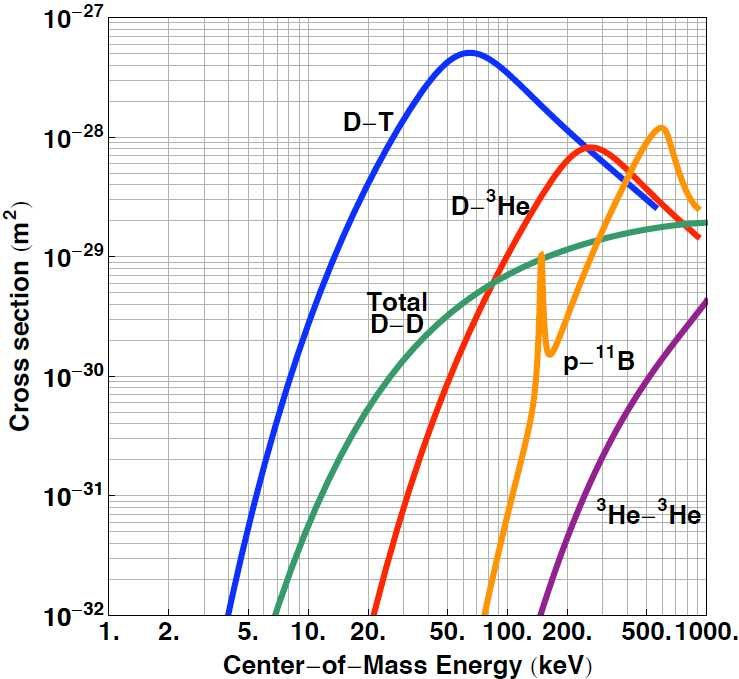
\includegraphics[width=.7\textwidth]{figures/fig_5.png}
    \caption{\it Fusion cross sections for various fusion reaction versus ion temperature. \cite{Moiraf2020}}
    \label{fig:fig_2_2}
\end{figure}
\\
\normalsize{\indent As said previously, the energies to achieve nuclear fusion are important. One solution to this problem is to give the correct amount of kinetic energy to the nuclei in order for them to overcome the Coulomb barrier. This kinetic energy is measured in Electron-Volts and is obtained by heating the fuel to high temperatures. The temperature thus reaches ~100M to 200M°C \cite{diekmann_energie:_2014}, which is hotter than the sun’s core. At those temperatures, the fuel becomes a plasma, which is often considered as the fourth state of matter. Plasma is also called the highest state of aggregation of a substance designated. In this aggregate state, the internal energy is far higher than the binding energy between the electrons and the nuclei. This means that the electrons can move freely. Plasma differs greatly in its properties from normal gases.}
\\
\break
\normalsize{\indent The important temperature of the plasma forces various measures to be taken to ensure that the Materials built into the fusion reactor near the plasma provide maintained thermal insulation and compensate for the resulting expansion pressure. A solution to this problem is the exploiting of the Lorenz force affecting the charged particles of the plasma. The idea is, at least for magnetic confinement, to trap the plasma inside a magnetic cage. This will help levitating the plasma and control its shape and position to avoid touching any \acrshort{PFCs}. The distance between the plasma and the \acrshort{PFCs} is crucial since contact could generate plasma turbulence or contaminate the plasma with impurities, reducing the quality of it. Different systems where developed to build such a confinement. }
\\
\break
\normalsize{\indent There are two different type of magnetic confinement concepts that are widely know and developed, the Tokamak and the Stellarator. These two magnetic confinement devices are both based on a toroidal geometry, the difference between the two of them being the way the plasma is confined. In a Tokamak machine, the plasma is confined using planar toroidal magnetic coils. Those coils help create the toroidal magnetic field component of the confinement. Although this seems like a good confinement, other problems still need to be addresses such as the effect of particle drift. This drift is due to  pressure gradients and inhomogeneities in the magnetic field inside the plasma and leads to a drift of the particles towards the outer diameter of the Tokamak. This complex particle transport phenomenon can be mitigated by introducing a poloidal component to the magnetic field, causing a rotation of the plasma around its toroidal axis. To achieve this magnetic field, Tokamaks use a solenoid coil placed at the center of the torus. This solenoid coil acts as a primary transformer coil, a time-varying electric current generate a varying magnetic field which itself induce an electric current inside the plasma. The resulting movement of charges inside the plasma generate a poloidal magnetic field, the plasma is then generating its own magnetic field. This electric current can also be used to heat up the plasma, it is called ohmic heating.}
\break
\begin{figure}[h!]
    \centering
    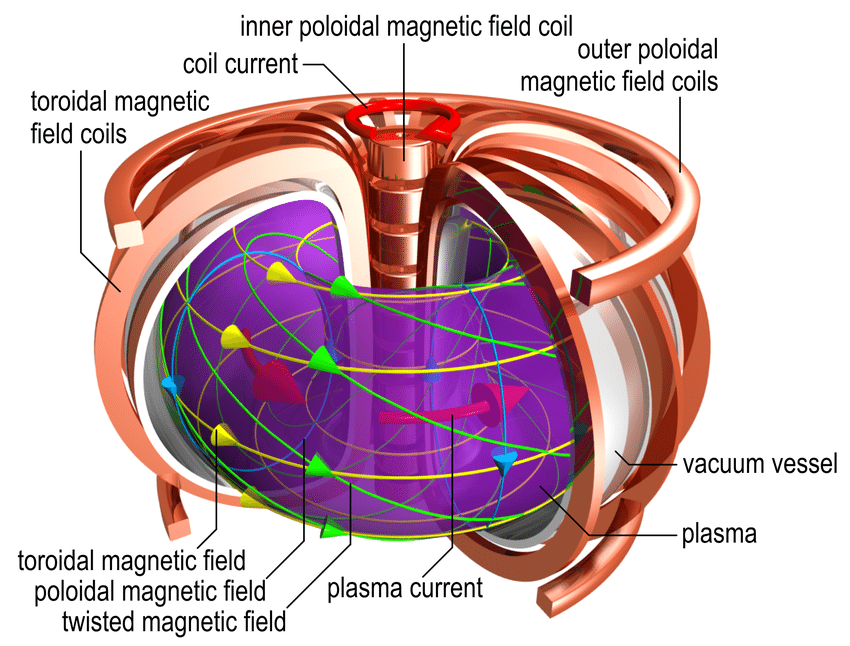
\includegraphics[width=.9\textwidth]{figures/fig_2.png}
    \caption{\it Schematics of a Tokamak confinement, courtesy of C. Brandt}
\end{figure}
\\
\break
\normalsize{\indent While this solution is good, there are problems with it. The main issue is the inherently transient process. The poloidal component of the magnetic field can only be generated as long as the current in the solenoid coil varies. This means that the reactor can only run in pulses and steady-state isn’t currently achievable.}
\\
\break
\normalsize{\indent Another solution for generating the poloidal magnetic field is to twirl the plasma in such a shape, that the drift phenomenon disappears. This solution is the Stellarator. The Stellarator was first introduced by Lyman Spitzer in the 1950s. This technology was put aside because of technical difficulties and because the Tokamaks presented better performances. The Stellarators use a complex set of magnets allowing to generate a precise magnetic field allowing the plasma to not experience significant drift. Contrary to Tokamaks, Stellerators plasmas don’t have a plasma current. This solution also helps with confinement, as the magnetic field can be adjusted to accommodate for the strict equilibrium conditions. The absence of plasma current also means that Stellarators can be operated in steady-state since no current induction is needed, thus being more suitable for power plants. Although allowing improved plasma confinement, Stellarators are plagues by complex geometries that are often too complex to be feasible.}
\begin{figure}[h!]
    \centering
    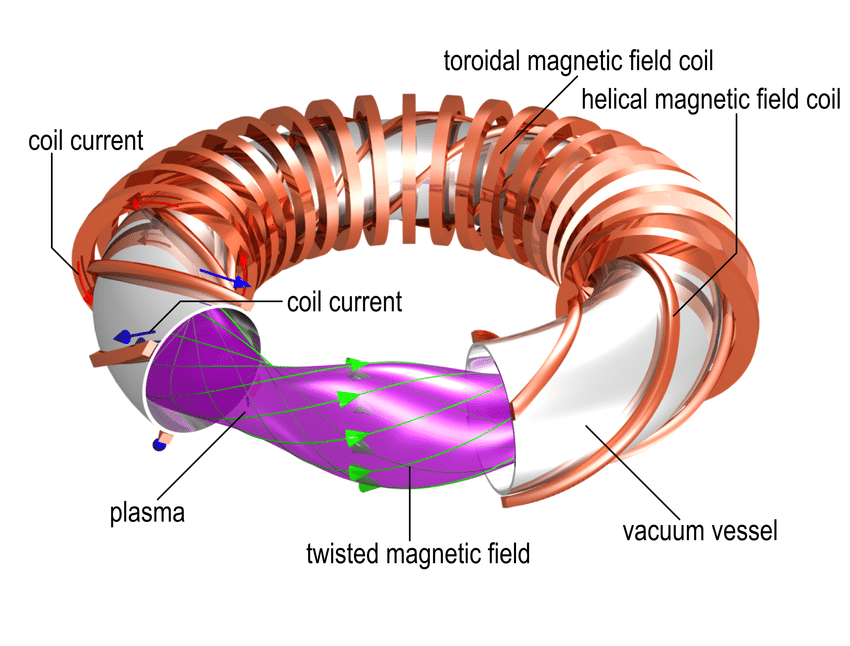
\includegraphics[width=.9\textwidth]{figures/fig_3.png}
    \caption{\it Schematics of a Stellarator confinement, courtesy of C. Brandt}
\end{figure}
\\
\normalsize{\indent The goal of those magnetic confinement fusion reactors concepts is to propose a new way of producing atomic energy while avoiding the drawbacks of traditional fission reactors (ie. Management of radiation, production of highly radioactive long half-life elements, limited fuel supply…). Although fusion energy is attractive, many problems still need to be addresses such as tritium breeding issues or neutron transport and interaction with the structure.}
\section{W7-X SYSTEMS}

\section{HEAT TRANSFER}
\normalsize{In this section, the fundamental principles and governing equations and each heat transfer mode are explored. The TZM-reflector tile is a highly constrained mechanical part that of the \acrshort{HS}. This part will be exposed to plasma radiation as well as the \acrshort{ECRH} beam.}




\section{SOLID MECHANICS}

\section{FINITE ELEMENT METHOD}

